%
% $RCSfile: whole_part.tex,v $
%
% Copyright (c) 2004. Christian Heller. All rights reserved.
%
% No copying, altering, distribution or any other actions concerning this
% document, except after explicit permission by the author!
% At some later point in time, this document is planned to be put under
% the GNU FDL license. For now, _everything_ is _restricted_ by the author.
%
% http://www.cybop.net
% - Cybernetics Oriented Programming -
%
% http://www.resmedicinae.org
% - Information in Medicine -
%
% @author Christian Heller <christian.heller@tuxtax.de>
%

\paragraph{Whole Part}
\label{whole_part_heading}

Whenever many components form a semantic unit, they can be subsumed by the
\emph{Whole-Part} pattern \cite{buschmann}. It encapsulates single part objects
(figure \ref{wholepart_figure}) and controls their cooperation. Part objects
are not addressable directly.

Almost all software systems contain components or sub systems which could be
organized by help of this pattern. In some way, it is quite similar to the
previously introduced \emph{Wrapper}, only that not just one- but many objects
are wrapped.

\begin{figure}[ht]
    \begin{center}
        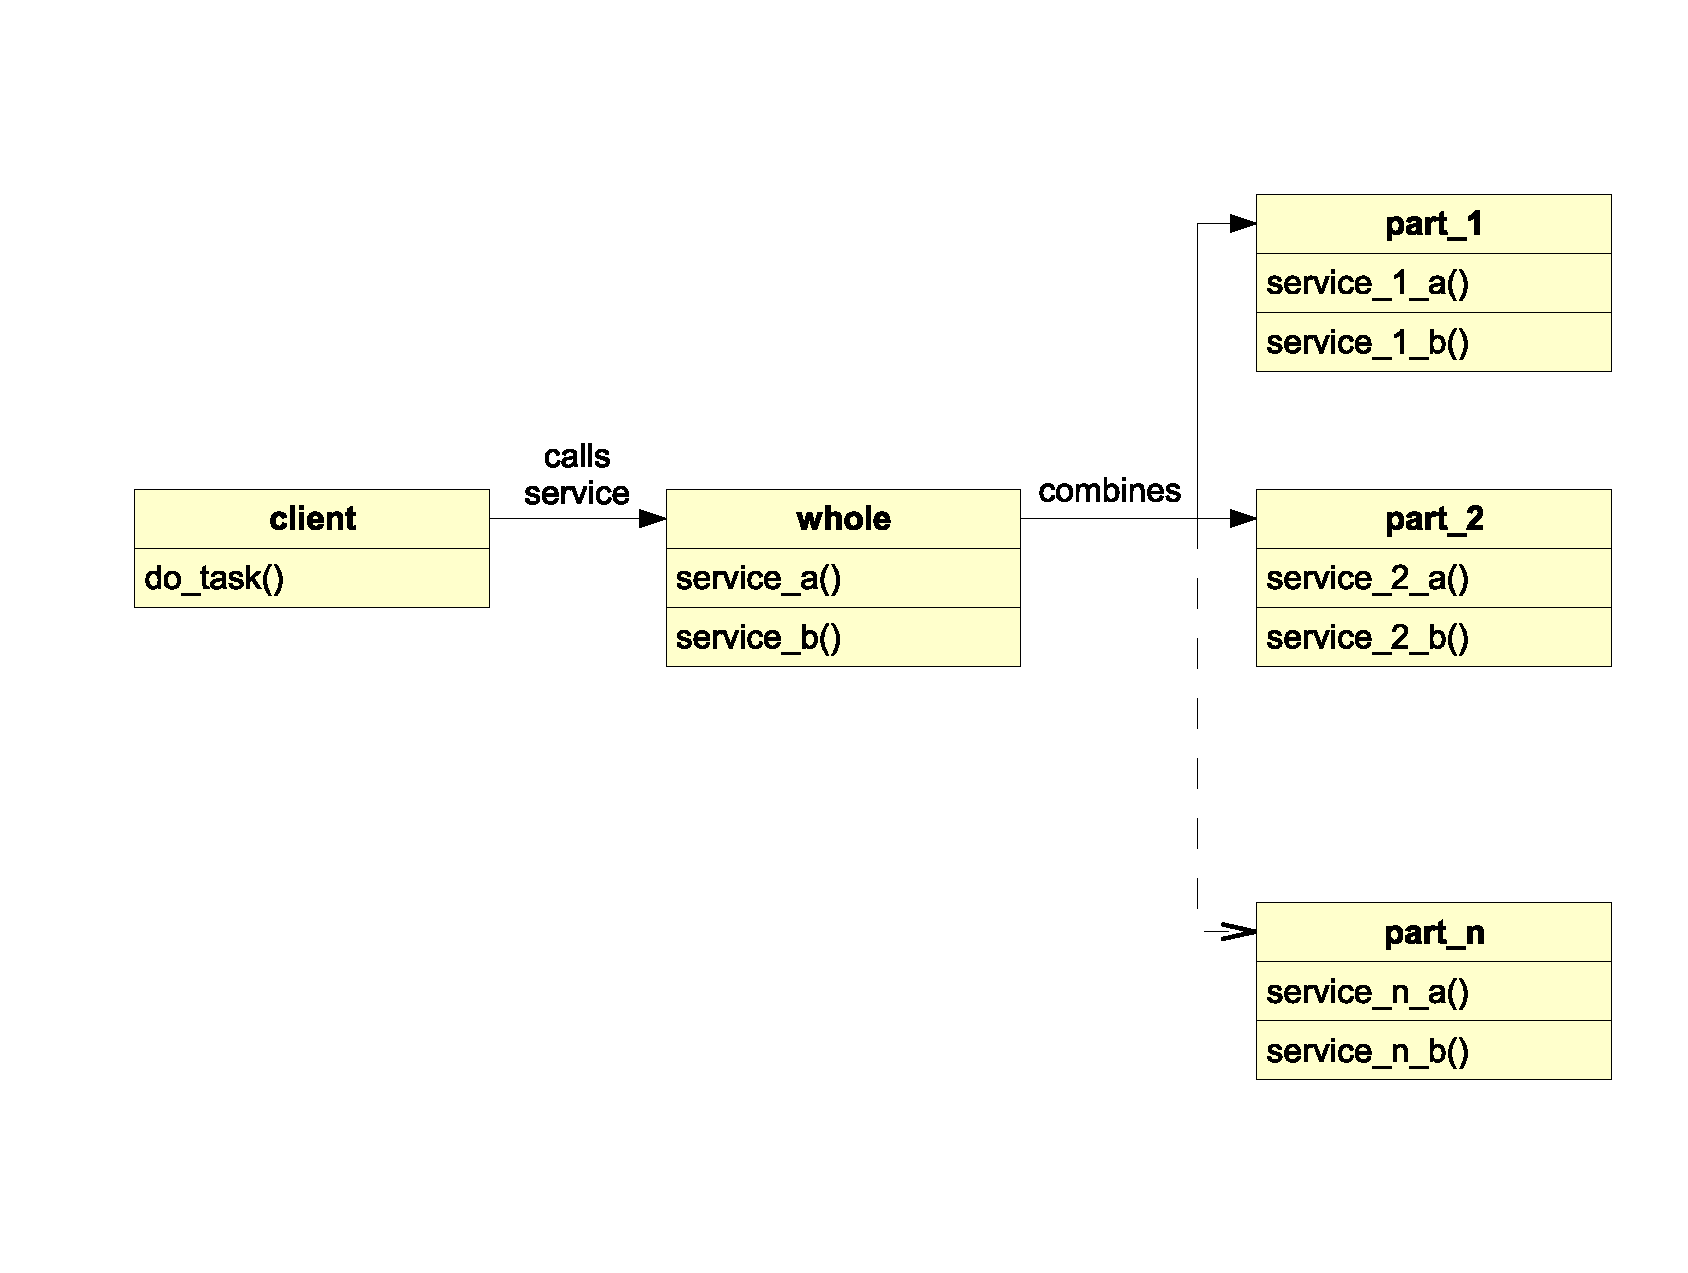
\includegraphics[scale=0.3]{vector/wholepart.eps}
        \caption{Whole-Part Pattern}
        \label{wholepart_figure}
    \end{center}
\end{figure}
